\documentclass{article}
\usepackage[utf8]{inputenc}
\usepackage{titling}
\usepackage{graphicx}
% Once I finish the ER diagram I'll add the images folder
\graphicspath{{./images/}}
\setlength{\droptitle}{-15em}
\title{CS450: Final }
\author{Emily Risley, Nicholas Grogg, Timothy Kudryn}
\date{04-28-2020}

\begin{document}

\maketitle

\section{Overview}

\subsection{Project design}

\subsection{Languages}

\subsection{Roles}

% Each person fills in their section
% Emily
\section{GUI}

% Tim
\section{Plots}

% Nick
\section{Backend}
\subsection{Web Server}
\noindent
For a web server, a web hosted CentOS 7 Linux server was used. This configuration was NOT a LAMP stack, as Apache and 
PHP were not used. Access was done via a user, password, IP and database combination by the front end. It was also 
possible to log into the server for maintenance using an SSH key, as password logins were disabled.

\subsection{Database}
\noindent
This database was a MariaDB database using the InnoDB engine. This engine was chosen as it's an atomic engine, so
transactions are either entirely successful or fail completely. 

\subsubsection{Database Values}
\noindent
Most of these values are somewhat obvious, however the FIPS (Federal Information Processing Standards) codes are not. 
These are unique numeric codes assigned by NIST (National Institute of Standards and Technology) assigned to states 
and counties. For this project only the two digits used for states were given in the dataset, with 
the three digit county FIPS numbers not included. \\ \\
\begin{tabular}{|l|l|}
	\hline
	Column & Description \\
	\hline
	Date & When the data was recorded \\
	\hline
	State & What state is the data from\\
	\hline
	FIPS & Two digit code used to identify a state \\
	\hline
	Cases & The number of recorded cases \\
	\hline
	Deaths & The number of readed deaths \\
	\hline
\end{tabular}

\subsubsection{ER Diagram}
\noindent
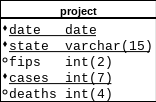
\includegraphics[scale=1]{erdiagram.png} \\
Underlined values are primary keys, these make up a composite primary key \\
Hollow symbols (Circles) are allowed to be NULL \\
Solid symbols (Diamonds) are not allowed to be NULL

\end{document}
